\documentclass[11pt]{article}

\usepackage{geometry}
\usepackage{amsthm}
\usepackage{amsmath}
\usepackage[utf8]{inputenc}
\usepackage{amsfonts}
\usepackage{lstfiracode}
\usepackage{fontspec}
\usepackage{enumitem}

\setmonofont{Fira Code}[
  Contextuals=Alternate
]
\newfontfamily{\firaseries}{Fira Code}
\usepackage{listings}
\usepackage{lstfiracode}
\lstset{
  language=Octave,
  basicstyle=\footnotesize\firaseries,
  numbers=none,
  showstringspaces=false,
  style=FiraCodeStyle,
  tabsize=2
}

\lstdefinelanguage{none}{
  identifierstyle=
}

\makeatletter
\lstdefinestyle{inline-style}{
  basicstyle=%
    \ttfamily
    \lst@ifdisplaystyle\scriptsize\fi
}
\makeatother

\newcommand*{\noaccsupp}[1]{\BeginAccSupp{ActualText={}}#1\EndAccSupp{}}

\newcommand\diagram[1]{
	\begin{center}
		\makebox[\textwidth]{\includegraphics[width=0.8\textwidth]{figures/#1}}
	\end{center}
}

\theoremstyle{definition}
\newtheorem{definition}{Definition}[section]
\newtheorem{example}[definition]{Example}
\newtheorem{problem}[definition]{Problem}
\newtheorem{claim}[definition]{Claim}
\newtheorem{observation}[definition]{Observation}
\newtheorem{notation}[definition]{Notation}

\begin{document}

\title{Problem Solving By Computer - Project 3}
\date{}
% \author{Jonathan Tang}
\maketitle

\section*{Introduction}
In the e-commerce world, there is an importance in being able to predict the behaviour of customers to survive in the market. In particular, is there a relation between a product being returned and the rating that was left by the customer? Moreover, are customers less likely to make future orders if they have previously returned a product for a refund? Finally, how can we determine the most valuable customers by deriving a ranking system which takes multiple attributes into account? \\

\noindent
In this project, we will analyse online transactions that were collected over four years for a given large online retailer. The data set is provided as a CSV (comma-separated values) file, and the first few lines of the data file are as follows. \\

\begin{lstlisting}
   Date      Customer_ID  Product_Category  Product_Value  Rating  Return
___________  ___________  ________________  _____________  ______  ______
01-Jan-2015    1010408           B              33.5         5       N 
01-Jan-2015    1014220           C              18.4         4       N 
01-Jan-2015    1016167           E              23.2         4       N 
01-Jan-2015    1019094           D                46         0       Y 
01-Jan-2015    1019535           D              25.5         0       N
\end{lstlisting}
$ $

\noindent
The schema of the data file is as follows.
\begin{lstlisting}[language=none]
Date: online transaction date (from 01 Jan 2015 to 31 Dec 2018)
Customer_ID: anonymised customer ID
Product_Category: one of 'A', 'B', 'C', 'D' or 'E'
Product_Value: the total amount of the order, in £GBP
Rating: the customer rating as a 1-5 star rating system, and 0 if no rating
Return: whether the product was returned for refund, N or Y
\end{lstlisting}

\noindent
We will start by reading the CSV file into a table. MATLAB uses type inference to determine the appropriate data types for the values in each column. In order to see the data types inferred by MATLAB, we can use the function \lstinline|summary(AllOrders)|.
\begin{lstlisting}
AllOrders = readtable('purchasing_order.csv');
summary(AllOrders)
\end{lstlisting}

\newpage
\section{Return rate on low rating items}
Since the majority of the customers who returned an order gave a low rating, we will start by finding a relation between the probability $P(r)$ that a product is likely to be returned and the rating $r$ the customer gave, using the following logistic function with two parameters $\alpha$ and $\beta$.

$$P(r) = \frac{1}{1 + \exp(-\alpha r - \beta)}$$

\noindent
That is, if the rating is low, then the customer is more likely to return the product. In order to reduce the overall computation complexity, we will only consider the ratings of those customers who have returned a product for refund.

\subsection{Preprocessing the data}
As we wish to only consider the ratings of those customers who have returned at least one product for refund, we first need to filter out orders from the data set that do not satisfy these requirements. It follows that we can first obtain the list of customer IDs for those who have returned a product for refund by first filtering for orders that were returned, then using MATLAB's \lstinline|unique()| function to remove any duplicates.

\begin{lstlisting}
ReturnedOrders = AllOrders(strcmp(AllOrders.Return, 'Y'), :);
Users_With_Returns = unique(ReturnedOrders.Customer_ID);
\end{lstlisting}

\noindent
Next, we need to obtain the orders that were placed by customers that have returned at least one order, and have a rating left by the customer. That is, we need to obtain the set of orders whose \lstinline|Customer_ID| belongs in the \lstinline|Users_With_Returns| list, and have \lstinline|Rating > 0|. We can obtain such subset of orders by using logical indexing as follows.

\begin{lstlisting}
Orders = AllOrders(ismember(AllOrders.Customer_ID, Users_With_Returns), :);
OrdersWithRatings = Orders(Orders.Rating > 0, :);
\end{lstlisting}

\noindent
That is, \lstinline|OrdersWithRating| contains orders from \lstinline|AllOrders| such that the customers who placed the orders have returned at least one product for refund.

\subsection{Finding the parameters $\alpha$ and $\beta$}
Suppose we have a function $f(\alpha, \beta)$ which tells us the lack of fit of the logistic function $P(r, \alpha, \beta)$, then we can minimise the lack of fit by using MATLAB's \lstinline|fminsearch()| function, which finds the minimum of a multi-variable function. That is, we can create an error function $f(\alpha, \beta)$ which tells us the lack of fit of the logisitic function $P(r)$ with parameters $\alpha$ and $\beta$, then use \lstinline|fminsearch()| to minimise the error.

\subsubsection{Models for the error function}
We will use the non-linear least squares model for our error function. As the name suggests, the error is given by the sum of the square of the errors. The non-linear least squares error function is as follows.

$$f(\alpha, \beta) = \sum_i \; \Big(p_i - P(r_i)\Big)^2 = \sum_i \; \Bigg(p_i - \frac{1}{1 + \exp(-\alpha r_i - \beta)}\Bigg)^2$$

\noindent
where $(r_i, p_i)$ is a transaction with rating $r_i \in [1, ..., 5]$ and a boolean flag $p_i \in \{0, 1\}$ which indicates whether the order was refunded, with 1 indicating that the order was refunded. \\

\noindent
The implementation of the non-linear least squares error function is as follows.

\begin{lstlisting}
function S = errorFunction(a, r, p)
  S = 0;
  for k = 1 : length(r)
    S = S + (p(k) - 1 / (1 + exp(-a(1) * r(k) - a(2))))^2;
  end
end
\end{lstlisting}

\noindent
It follows that we can use find the parameters $\alpha$ and $\beta$ by minimising the error function.

\begin{lstlisting}
orderRating = OrdersWithRatings.Rating;
orderIsReturned = strcmp(OrdersWithRatings.Return, 'Y');
lrParams = fminsearch(@(a) errorFunction(a, orderRating, orderIsReturned), [0 0]);
fprintf('α = %.5f, β = %.5f\n', lrParams); 
\end{lstlisting}

\subsection{Results}

We conclude that the relation between the probability $P(r)$ that a product is likely to returned and the rating $r$ the customer gave, is governed by the following logistic function.

$$P(r) = \frac{1}{1 + \exp(17.542411 r - 17.418797)}$$

\noindent
That is, we conclude that the parameters are $\alpha = -17.542411$ and $\beta = 17.418797$. Moreover, we can plot the logistic function against the data points as follows.

\begin{lstlisting}
hx = linspace(0, 6, 1001);
plot(orderRating, isOrderReturned, 'o', ...
     hx, 1 ./ (1 + exp(-lrParams(1) * hx - lrParams(2))));
lg = legend('Raw Data', 'Logistic Regression');
set(lg,'Location', 'east');
xlabel('Rating'); xticks([1 : 5]);
ylabel('Order Returned'); yticks([0, 1]); yticklabels({'No', 'Yes'});
axis([0.5, 5.5, -0.1, 1.1]);
\end{lstlisting}

\diagram{logistic_function}

% TODO: Conclusion on the parameters and what they mean

\newpage
\section{Modelling moving interceptors}

Suppose we wish to fire the cannonballs to destroy a target at 15000 meters away. However, there are interceptors located at 12000 meters away, which are being fired vertically at regular intervals, which could block the cannonballs. Each interceptor is 1000 meters long, is launched every 20 seconds, and moves upward with uniform velocity. The initial configuration at time $t = 0$ is shown below.\\

\noindent
\textbf{Question:} What are the possible firing angles and associated firing times, such that the cannonball will destroy the target without being blocked by an interceptor?

\begin{center}
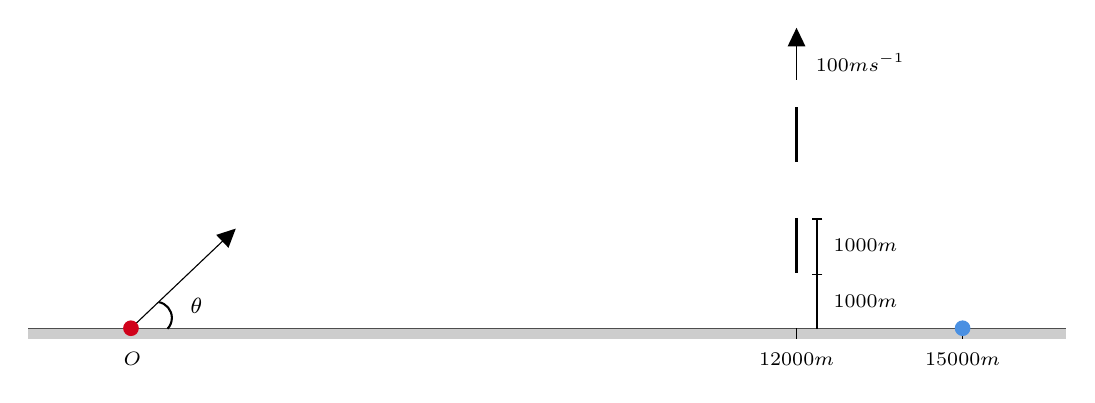
\begin{tikzpicture}[x=0.75pt,y=0.75pt,yscale=-1,xscale=1]

%Straight Lines [id:da45198010726670845] 
\draw    (80.33,155) -- (580.33,155) ;
%Shape: Rectangle [id:dp9890398319964502] 
\draw  [draw opacity=0][fill={rgb, 255:red, 155; green, 155; blue, 155 }  ,fill opacity=0.5 ] (80.33,155) -- (580.33,155) -- (580.33,160.33) -- (80.33,160.33) -- cycle ;
%Straight Lines [id:da9896789843028051] 
\draw    (129.83,155) -- (178.16,109.07) ;
\draw [shift={(180.33,107)}, rotate = 496.45] [fill={rgb, 255:red, 0; green, 0; blue, 0 }  ][line width=0.08]  [draw opacity=0] (8.93,-4.29) -- (0,0) -- (8.93,4.29) -- cycle    ;
%Shape: Arc [id:dp2518682859253052] 
\draw  [draw opacity=0][line width=0.75]  (143.2,142.42) .. controls (146.79,143.06) and (149.52,146.19) .. (149.54,149.96) .. controls (149.55,152.02) and (148.76,153.88) .. (147.45,155.27) -- (141.84,150) -- cycle ; \draw  [line width=0.75]  (143.2,142.42) .. controls (146.79,143.06) and (149.52,146.19) .. (149.54,149.96) .. controls (149.55,152.02) and (148.76,153.88) .. (147.45,155.27) ;
%Shape: Circle [id:dp13299007709992905] 
\draw  [color={rgb, 255:red, 208; green, 2; blue, 27 }  ,draw opacity=1 ][fill={rgb, 255:red, 208; green, 2; blue, 27 }  ,fill opacity=1 ] (126.33,155) .. controls (126.33,153.07) and (127.9,151.5) .. (129.83,151.5) .. controls (131.77,151.5) and (133.33,153.07) .. (133.33,155) .. controls (133.33,156.93) and (131.77,158.5) .. (129.83,158.5) .. controls (127.9,158.5) and (126.33,156.93) .. (126.33,155) -- cycle ;
%Straight Lines [id:da7363174446974949] 
\draw    (450.5,155.13) -- (450.5,160.13) ;
%Straight Lines [id:da8507054156705689] 
\draw    (530.5,155.13) -- (530.5,160.13) ;
%Shape: Circle [id:dp0875287559905249] 
\draw  [color={rgb, 255:red, 74; green, 144; blue, 226 }  ,draw opacity=1 ][fill={rgb, 255:red, 74; green, 144; blue, 226 }  ,fill opacity=1 ] (527,155) .. controls (527,153.07) and (528.57,151.5) .. (530.5,151.5) .. controls (532.43,151.5) and (534,153.07) .. (534,155) .. controls (534,156.93) and (532.43,158.5) .. (530.5,158.5) .. controls (528.57,158.5) and (527,156.93) .. (527,155) -- cycle ;
%Straight Lines [id:da9565901506094769] 
\draw [line width=1.25]    (450.5,101.79) -- (450.5,128.46) ;
%Straight Lines [id:da8590807071227391] 
\draw [line width=1.25]    (450.5,48.46) -- (450.5,75.12) ;
%Straight Lines [id:da1250805630667582] 
\draw [line width=0.5]    (460.36,102.39) -- (460.36,129.06) ;
%Straight Lines [id:da2542517178085071] 
\draw [line width=0.5]    (462.94,102.39) -- (457.77,102.39) ;
%Straight Lines [id:da9006595888470921] 
\draw [line width=0.5]    (462.94,129.06) -- (457.77,129.06) ;

%Straight Lines [id:da4594515235335257] 
\draw [line width=0.5]    (460.36,129.06) -- (460.36,155.3) ;
%Straight Lines [id:da8735781741018898] 
\draw [line width=0.5]    (450.5,13.25) -- (450.5,35.46) ;
\draw [shift={(450.5,10.25)}, rotate = 90] [fill={rgb, 255:red, 0; green, 0; blue, 0 }  ][line width=0.08]  [draw opacity=0] (8.93,-4.29) -- (0,0) -- (8.93,4.29) -- cycle    ;

\draw (161.33,144) node  [font=\footnotesize]  {$\theta$};
\draw (450.5,170) node  [font=\scriptsize]  {$12000m$};
\draw (530.5,170) node  [font=\scriptsize]  {$15000m$};
\draw (483.7,115.2) node  [font=\scriptsize]  {$1000m$};
\draw (483.7,142.18) node  [font=\scriptsize]  {$1000m$};
\draw (481.2,26.85) node  [font=\scriptsize]  {$100ms^{-1}$};
\draw (130.5,170) node  [font=\scriptsize]  {$O$};

\end{tikzpicture}
\end{center}


\subsection{Finding the required firing angles to reach the target}
First, we observe that the firing angle required to yield a given horizontal displacement is independent of the firing time. As a result, we can start by finding the firing angles in order to reach the target horizontal displacement of 15000m. Using our \lstinline|distance_function|, we can plot the horizontal displacement against the associated firing angle as follows.

\begin{lstlisting}
distance = @(theta) distance_function(g, v, m, K, theta);

angles = linspace(0, pi / 2, 100);
displacement = arrayfun(distance, angles);
displacement(1) = 0;

plot(angles, displacement);
title('Horizontal Displacement vs Firing Angle');
xlabel('Firing Angle (degrees)');
ylabel('Horizontal Displacement (m)');
yline(15000);

% Remove exponential notation from axis tick labels
ax = gca;
ax.YAxis.Exponent = 0;
\end{lstlisting}

\noindent
For our chosen model parameters ($g = 9.8, \; v = 450, \; m = 6, \; K = 0.00002$), the plot for the horizontal displacement against the associated firing angle is shown below.
\diagram{angle_vs_displacement}

\noindent
By looking at the plot, we see that the distance function $f_{x}(\theta)$ is a unimodal function. That is, $f_{x}(\theta)$ is increasing on $[0, \theta_{max}]$, and decreasing on $[\theta_{max}, \pi / 2]$, where $\theta_{max}$ is the firing angle that yields the maximum horizontal displacement. In particular, suppose we wish to hit a target at distance $d$, then, there are three possible outcomes:
\begin{enumerate}
	\item If $d > f_x(\theta_{max})$, then it is impossible to hit the target.
	\item If $d = f_x(\theta_{max})$, then $\theta_{max}$ is precisely the only firing angle to reach this distance.
	\item If $d < f_x(\theta_{max})$, then there are two solutions to the equation $f_x(\theta) = d$. One solution lies in the interval $(0, \theta_{max})$, and the other lies in the interval $(\theta_{max}, \pi / 2)$.
\end{enumerate}

\noindent
Earlier, we saw that the firing angle which yields the maximum horizontal displacement is $\theta_{max} = 0.778422$ with $f_x(\theta_{max}) = 19617.77$m. As the distance of our target, 15000m, is less than the maximum distance, we have two possible firing angles, which can be found using the \lstinline|fzero| function provided by MATLAB. Indeed, we can use \lstinline|fzero| to find the values of $\theta$ where the distance function $f_x(\theta)$ and the line $y = 15000$ intersect, by finding the roots of $f_{15000}(\theta) = f_x(\theta) - 15000$. The implementation of finding the firing angles is as follows.

\begin{lstlisting}
target_distance = 15000;
distance_fun = @(theta) distance_function(g, v, m, K, theta);
[maxTheta, ~] = fminbnd(@(theta) -distance_fun(theta), 0, pi / 2);

distance_from_target = @(theta) distance_fun(theta) - target_distance;
thetaOne = fzero(distance_from_target, [eps, maxTheta]);
thetaTwo = fzero(distance_from_target, [maxTheta, pi / 2]);
\end{lstlisting}

\noindent
We conclude that the two firing angles which yield a horizontal distance of 15000m are $\theta_1 = 0.425366$ and $\theta_2 = 1.133637$. The trajectory plots for $\theta_1$ and $\theta_2$ are shown below.

\diagram{firing_angles}

\subsection{Finding the time and height for a given horizontal displacement}
In order to determine whether the trajectory of the cannonball is blocked by the interceptor, we need to know the height of the cannonball when the distance travelled by the ball is 12000m. As the interceptors are moving, we also need to know the time taken for the cannonball to reach the horizontal distance of 12000m. In order to do this, we can add a non-terminating event to our event function, which we can use to obtain the time and height at which the cannonball arrives at the interceptors. We can add a second event to our event function as follows.

\begin{lstlisting}
function [value, isTerminal, direction] = events_function(t, z, distance)
  value(1) = z(1) - distance;    % When the distance is 12000,
  isTerminal(1) = 0;             % take note of the event.
  direction(1) = 1;
  
  value(2) = z(2);               % When the height is 0,
  isTerminal(2) = 1;             % terminate integration,
  direction(2) = -1;             % but only if the ball is falling
end
\end{lstlisting}

\noindent
Notice that, for this event, we set \lstinline|isTerminal = 0| to indicate that we only want to detect when this event occurs, rather than halt integration when this event occurs.

\newpage
\noindent
Consequently, we need to update our \lstinline|projection_solution| function to take into account the \lstinline|distance| parameter, as follows. Notice that on Line 5, we use a similar design pattern as earlier, by using \lstinline|events_function(t, z, distance)| to generate \lstinline|events_fun(t, z)|.

\begin{lstlisting}
function [t, z, te, ze] = projection_solution(g, v, m, K, theta, distance)
  ode = @(t, z) projection_ode(t, z, g, m, K);
  tspan = [0, 2 * v / g];
  ic = [0, 0, v * cos(theta), v * sin(theta)];
  events_fun = @(t, z) events_function(t, z, distance);
  options = odeset('events', events_fun, 'reltol', 1e-8);
  [t, z, te, ze] = ode45(ode, tspan, ic, options);
end
\end{lstlisting}

\noindent
Finally, we can obtain the information (time and height of cannonball) about the event at which the cannonball arrives at the interceptors, as follows.

\begin{lstlisting}
ic_distance = 12000;
[t1, z1, te1, ze1] = projection_solution(g, v, m, K, thetaOne, ic_distance);
[t2, z2, te2, ze2] = projection_solution(g, v, m, K, thetaTwo, ic_distance);

fprintf('[theta = %.4f]: %.4fs to reach %dm, with height %.4fm\n', ...
        thetaOne, te1(1), ic_distance, ze1(1, 2));
fprintf('[theta = %.4f]: %.4fs to reach %dm, with height %.4fm\n', ...
        thetaTwo, te2(1), ic_distance, ze2(1, 2));
\end{lstlisting}

\noindent
We conclude that by firing at angle $\theta_1 = 0.425366$, it takes $t_1 = 29.8907$s to reach a distance of 12000m, with height $y_1 = 1117.1270$m. Likewise, if we fire at angle $\theta_2 = 1.133637$, it takes $t_2 = 65.0186$s to reach a distance of 12000m, with height $y_2 = 5318.9654$m.

\subsection{Finding the firing times to avoid the interceptors}
All that remains in order to find the firing times such that the trajectory of the cannonball avoids the interceptors, is to model the interceptors. That is, we need to determine whether an interceptor is present, for a given time and height. It turns out that we can model the positions of the interceptors by a system of inequalities, as shown in the figure below.

\begin{center}
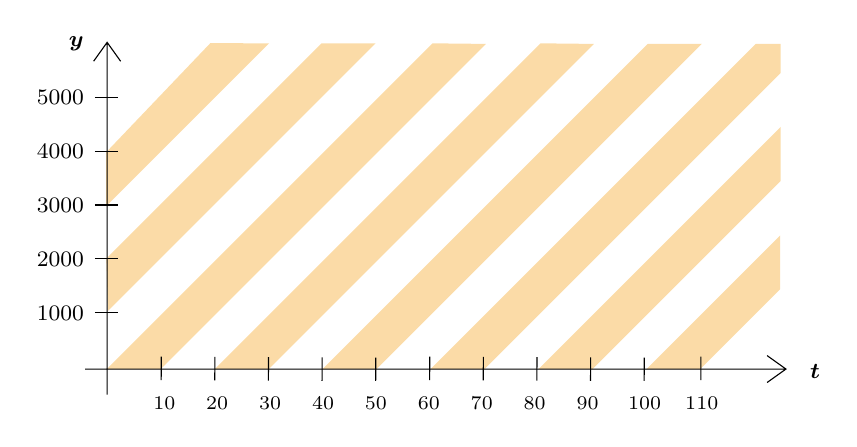
\begin{tikzpicture}[x=0.75pt,y=0.75pt,yscale=-1.3,xscale=1.3]

%Straight Lines [id:da8684061662750675] 
\draw [draw opacity=0][fill={rgb, 255:red, 245; green, 166; blue, 35 }  ,fill opacity=0.4 ]   (290.11,10.03) -- (210.33,89.81) -- (210.94,109.19) -- (310.11,10.03) ;
%Straight Lines [id:da20070134274560436] 
\draw [draw opacity=0][fill={rgb, 255:red, 245; green, 166; blue, 35 }  ,fill opacity=0.4 ]   (331.22,10.03) -- (210.5,130.75) -- (230.5,130.75) -- (351,10.25) ;
%Straight Lines [id:da15667199057255] 
\draw [draw opacity=0][fill={rgb, 255:red, 245; green, 166; blue, 35 }  ,fill opacity=0.4 ]   (371.22,10.03) -- (250.5,130.75) -- (270.5,130.75) -- (391,10.25) ;
%Straight Lines [id:da16111006653858873] 
\draw [draw opacity=0][fill={rgb, 255:red, 245; green, 166; blue, 35 }  ,fill opacity=0.4 ]   (411.05,10.2) -- (290.5,130.75) -- (310.5,130.75) -- (431,10.25) ;
%Straight Lines [id:da17132951955454145] 
\draw [draw opacity=0][fill={rgb, 255:red, 245; green, 166; blue, 35 }  ,fill opacity=0.4 ]   (451.05,10.2) -- (330.5,130.75) -- (350.5,130.75) -- (460.25,21) -- (460.2,10.2) ;
%Straight Lines [id:da7059801466329929] 
\draw [draw opacity=0][fill={rgb, 255:red, 245; green, 166; blue, 35 }  ,fill opacity=0.4 ]   (460.25,41) -- (370.5,130.75) -- (390.5,130.75) -- (460.2,61.05) ;
%Straight Lines [id:da1725362087062552] 
\draw [draw opacity=0][fill={rgb, 255:red, 245; green, 166; blue, 35 }  ,fill opacity=0.4 ]   (460.05,81.2) -- (410.5,130.75) -- (430.5,130.75) -- (460.05,101.2) ;
%Straight Lines [id:da9555245018524643] 
\draw [draw opacity=0][fill={rgb, 255:red, 245; green, 166; blue, 35 }  ,fill opacity=0.4 ]   (210.27,70.4) -- (270.61,10.06) -- (248.9,9.93) -- (210.27,50.4) ;

%Shape: Axis 2D [id:dp34426191300315345] 
\draw  (202.5,130.75) -- (462.2,130.75)(210.62,9.67) -- (210.62,140.25) (455.2,125.75) -- (462.2,130.75) -- (455.2,135.75) (205.62,16.67) -- (210.62,9.67) -- (215.62,16.67)  ;
%Straight Lines [id:da687805521470227] 
\draw    (206.08,30.17) -- (214.75,30.17) ;
%Straight Lines [id:da29463863993196715] 
\draw    (206.08,89.81) -- (214.75,89.81) ;
%Straight Lines [id:da23889549179341274] 
\draw    (206.08,50.05) -- (214.75,50.05) ;
%Straight Lines [id:da8827821095526927] 
\draw    (206.08,109.67) -- (214.75,109.67) ;
%Straight Lines [id:da14240699948891322] 
\draw    (206.08,69.93) -- (214.75,69.93) ;

%Straight Lines [id:da13236081794663002] 
\draw    (310.19,126.51) -- (310.15,135.17) ;
%Straight Lines [id:da6764330802644254] 
\draw    (250.55,126.25) -- (250.51,134.91) ;
%Straight Lines [id:da2195181324463853] 
\draw    (290.31,126.42) -- (290.27,135.09) ;
%Straight Lines [id:da40738199528142127] 
\draw    (230.69,126.16) -- (230.65,134.83) ;
%Straight Lines [id:da834666862936023] 
\draw    (270.43,126.33) -- (270.39,135) ;
%Straight Lines [id:da8176799234123608] 
\draw    (409.69,126.51) -- (409.65,135.17) ;
%Straight Lines [id:da0901662764399862] 
\draw    (350.05,126.25) -- (350.01,134.91) ;
%Straight Lines [id:da7280602976758792] 
\draw    (389.81,126.42) -- (389.77,135.09) ;
%Straight Lines [id:da4515893530436432] 
\draw    (330.19,126.16) -- (330.15,134.83) ;
%Straight Lines [id:da7435564988815735] 
\draw    (369.93,126.33) -- (369.89,135) ;
%Straight Lines [id:da11328121299548322] 
\draw    (430.69,126.16) -- (430.65,134.83) ;

% Text Node
\draw (193.31,70.17) node  [font=\footnotesize]  {$3000$};
% Text Node
\draw (193.31,50.17) node  [font=\footnotesize]  {$4000$};
% Text Node
\draw (193.31,110.17) node  [font=\footnotesize]  {$1000$};
% Text Node
\draw (193.31,90.17) node  [font=\footnotesize]  {$2000$};
% Text Node
\draw (193.31,30.17) node  [font=\footnotesize]  {$5000$};
% Text Node
\draw (473.01,131.47) node  [font=\footnotesize]  {$\boldsymbol{t}$};
% Text Node
\draw (231.81,143.5) node  [font=\scriptsize]  {$10$};
% Text Node
\draw (251.42,143.5) node  [font=\scriptsize]  {$20$};
% Text Node
\draw (271.03,143.5) node  [font=\scriptsize]  {$30$};
% Text Node
\draw (290.64,143.5) node  [font=\scriptsize]  {$40$};
% Text Node
\draw (310.25,143.5) node  [font=\scriptsize]  {$50$};
% Text Node
\draw (329.86,143.5) node  [font=\scriptsize]  {$60$};
% Text Node
\draw (349.47,143.5) node  [font=\scriptsize]  {$70$};
% Text Node
\draw (388.69,143.5) node  [font=\scriptsize]  {$90$};
% Text Node
\draw (369.08,143.5) node  [font=\scriptsize]  {$80$};
% Text Node
\draw (409.81,143.5) node  [font=\scriptsize]  {$100$};
% Text Node
\draw (431.01,143.5) node  [font=\scriptsize]  {$110$};
% Text Node
\draw (199.21,10.27) node  [font=\footnotesize]  {$\boldsymbol{y}$};

\end{tikzpicture}
\end{center}


\noindent
The shaded regions indicate the presence of an interceptor, whereas the the non-shaded regions indicate the absence of an interceptor. Each shaded region is defined by two lines, the line to the left of the shaded region which indicates the top of the interceptor, and the line to the right of the shaded region which indicates the bottom of the interceptor.\\

\noindent
Observe that the gradient of the lines are 100 and every lower bound line passes through the point $(20n, 0)$, so the lower bound lines are of the form $y = 100(t - 20n)$, $n \in \mathbb{N} \cup \{0\}$. In order to find the maximum delay before firing the cannonball such that the cannonball misses the interceptor, we need to find the point $(t_d, h_i)$, where $t_d$ lies on a lower bound line and $t_i \leq t_d$.

\begin{center}
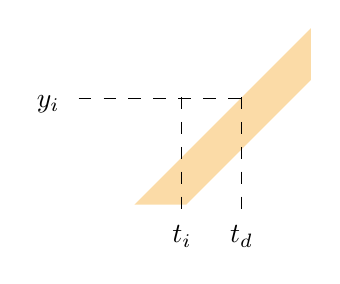
\begin{tikzpicture}[x=0.75pt,y=0.75pt,yscale=-1.25,xscale=1.25]
%Straight Lines [id:da44466472645933863] 
\draw [draw opacity=0][fill={rgb, 255:red, 245; green, 166; blue, 35 }  ,fill opacity=0.4 ]   (385.5,9.75) -- (317.5,77.75) -- (337.5,77.75) -- (385.5,29.75) ;
%Straight Lines [id:da19295940989666804] 
\draw  [dash pattern={on 4.5pt off 4.5pt}]  (296,36.75) -- (358.65,36.75) ;
%Straight Lines [id:da33383227408636085] 
\draw  [dash pattern={on 4.5pt off 4.5pt}]  (335.65,36.25) -- (335.65,81.67) ;
%Straight Lines [id:da7914567806567081] 
\draw  [dash pattern={on 4.5pt off 4.5pt}]  (358.65,36.25) -- (358.65,81.67) ;


% Text Node
\draw (284.31,39) node  [font=\normalsize] {$y_i$};
% Text Node
\draw (335.81,90) node  [font=\normalsize] {$t_i$};
% Text Node
\draw (358.81,90) node  [font=\normalsize] {$t_d$};

\end{tikzpicture}
\end{center}

\noindent
Putting the equation of the lower bound line and the inequality together, we have
$$\frac{1}{20}\Bigg(t_i - \frac{y_i}{100}\Bigg) \leq n.$$
However, as $n$ is an integer, we can find the least such $n$ that satisfies the inequality by 
$$n = \Bigg\lceil \frac{1}{20}\Bigg(t_i - \frac{y_i}{100}\Bigg) \Bigg\rceil.$$
It follows that $t_d = 0.01 y_i + 20n$ and so the maximum delay we can wait before firing the cannonball is given by $t_d - t_i$. If $(t_i, y_i)$ lies in a shaded region, we need to calculate a minimum delay that we must wait before firing the cannonball. Observe that if the maximum delay is less than 10, then $(t_i, y_i)$ must lie in a non-shaded region, otherwise, the minimum delay can be computed by $t_d - t_i - 10$. However, for our parameters, it turns out that both $(t_1, y_1)$ and $(t_2, y_2)$ lie outside the shaded region, and so the minimum delay is 0. The implementation of finding the maximum delay is as follows.

\begin{lstlisting}
function d = delay_function(t, h)
  n = ceil(0.05 * (t - 0.01 * h));
  td = 0.01 * h + 20 * n - t;
  d = [max(td - 10, 0), td];
end
\end{lstlisting}

\newpage
\noindent
We find the intervals of delay for $\theta_1$ and $\theta_2$ as follows.
\begin{lstlisting}
ic_distance = 12000;
[t1, z1, te1, ze1] = projection_solution(g, v, m, K, thetaOne, ic_distance);
[t2, z2, te2, ze2] = projection_solution(g, v, m, K, thetaTwo, ic_distance);
      
d1 = delay_function(te1(1), ze1(1, 2));
d2 = delay_function(te2(1), ze2(1, 2));
      
fprintf('[theta = %.4f]: Min Delay = %.4f, Max Delay = %.4f\n', ...
        thetaOne, d1(1), d1(2));
fprintf('[theta = %.4f]: Min Delay = %.4f, Max Delay = %.4f\n', ...
        thetaTwo, d2(1), d2(2));
\end{lstlisting}

\noindent
The above code snippet produces the following output.
\begin{lstlisting}
[theta = 0.4254]: Min Delay = 0.0000, Max Delay = 1.2805
[theta = 1.1336]: Min Delay = 0.0000, Max Delay = 8.1711
\end{lstlisting}

\noindent
We conclude that in order to fire with launch angle $\theta_1 = 0.425366$ without hitting any interceptors, we can fire at times $t \in [0, 1.2805)$. However, as the interceptors are fired periodically every 20 seconds, with the interceptor and the gap being of equal width, we can also fire every other 10 seconds after 1.2805. That is, for $\theta_1 = 0.425366$, we can fire at times $t \in (11.2805, 21.28025) \cup (31.28025, 41.28025) \cup \dots \cup (11.2805 + 20n, 21.2805 + 20n)$. \\

\noindent
Similarly, in order to avoid the interceptors when firing with launch angle $\theta_2 = 1.133637$, we can fire at times $t \in [0, 8.1711) \cup (18.1711, 28.1711) \cup \dots \cup (18.1711 + 20n, 28.1711 + 20n)$.

\subsection{Results}
\noindent
We have found the two possible launch angles and the associated firing times, such that the cannonball will hit the target placed 15000m away, without being blocked by an interceptor.
$$\theta_1 = 0.425366, \; t_{\theta_1} = [0, 1.2805) \cup \{(11.2805 + 20n, 21.2805 + 20n) \; \vert \; n \in \mathbb{N} \cup \{0\}\}$$
$$\theta_2 = 1.133637, \; t_{\theta_2} = [0, 8.1711) \cup \{(18.1711 + 20n, 28.1711 + 20n) \; \vert \; n \in \mathbb{N} \cup \{0\}\}$$




\end{document}
